
\begin{frame}[c]{Modell der Selbstmanagement-Kompetenz}
    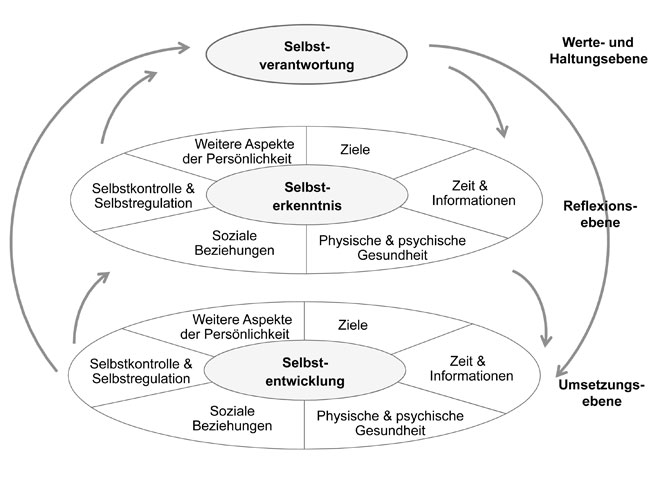
\includegraphics[width=\textwidth]{zsm/modell.jpeg}
\end{frame}


\section{Selbstverantwortung}

\begin{frame}[c]{Selbstverantwortung - Verhaltensindikatoren}
    \begin{itemize}
    \item Persönliche Lebensphilosophie
    \pause
    \item Verantwortung für eigenes Leben und Lebensführung übernehmen
    \pause
    \item Schuld für Missstände nicht externalisieren
    \pause
    \item Sich über Selbst- und Fremdbestimmung bewusst sein
    \end{itemize}
\end{frame}


\begin{frame}[c]{Selbstverantwortung - Reflektionsfragen}
    \begin{itemize}
    \item Was ist mir im Leben am wichtigsten? \newline
    \pause
    \item Wirkt sich Fremdbestimmung negativ auf mein Wohlbefinden aus? \newline
    \pause
    \item Übernehme ich genug Verantwortung für mein Wohlbefinden?
    \end{itemize}
\end{frame}


\begin{frame}[standout]
    Was wünsche ich mir für meine Zukunft?
\end{frame}





\section{Selbsterkenntnis}

\begin{frame}[c]{Selbsterkenntnis - Verhaltensindikatoren}
    \begin{itemize}
    \item Erkenntnisgewinn über das eigene Selbst (Realistische Reflektion) \newline
    \pause
    \item Bewusstsein für das eigene Verhalten entwickeln \newline
    \pause
    \item Erkennen und akzeptieren eigener Schwächen \newline
    \end{itemize}
\end{frame}


\begin{frame}[c]{Selbsterkenntnis - Reflektionsfragen}
    \begin{itemize}
    \item Was sagt mir mein Körper wie es mir geht? \newline
    \pause
    \item Was kann ich gut? \newline
    \pause
    \item Welche Einstellungen und Verhaltensmuster prägen mich?
    \end{itemize}
\end{frame}


\begin{frame}[standout]
    \huge
    Tagesreflektion
\end{frame}





\section{Selbstentwicklung}

\begin{frame}[c]{Selbstentwicklung - Verhaltensindikatoren}
    \begin{itemize}
    \item Weiterentwicklung der Persönlichkeit mit dem Verlauf des Lebens
    \pause
    \item Klares Hinarbeiten auf eigene Ziele
    \pause
    \item Offenheit neuen Erfahrungen gegenüber erhalten
    \pause
    \item Eigene Einstellung verändern können
    \end{itemize}
\end{frame}


\begin{frame}[c]{Selbstentwicklung - Reflektionsfragen}
    \begin{itemize}
    \item Was will ich im Leben noch erfahren/lernen/wissen? \newline
    \pause
    \item Wo schränke ich mich in meinen Möglichkeiten selbst ein? \newline
    \pause
    \item Wie ist meine Körperhaltung jetzt gerade?
    \end{itemize}
\end{frame}


\begin{frame}[standout]
    Übung
\end{frame}





\section{Ziele}

\begin{frame}[c]{Ziele - Anwendung}
    \begin{itemize}
    \item Persönliche Ziele definieren und analysieren \pause Wichtig: Realisierbarkeit
    \pause
    \item Zielkonflikte erkennen und behandeln
    \pause
    \item Konkrete Handlungspläne für die Zielerreichung umfassend ausgestalten
    \pause
    \item Entschlossen an Zielen festhalten
    \end{itemize}
\end{frame}





\section{Zeit und Informationen}

\begin{frame}[c]{Zeitmanagement}
    \begin{itemize}
    \item Zeit bewusst und zielorientiert einteilen \newline
    \pause
    \item Erholung gezielt in den Zeitplan integrieren \newline
    \pause
    \item Zeitdiebe elimieren
    \end{itemize}
\end{frame}



\section{Physische und Psychische Gesundheit}

\begin{frame}[c]{Gesundheit}
    \begin{itemize}
    \item Bewusstsein für die Wichtigkeit des eigenen physischen und psychischen Zustands entwickeln \newline
    \pause
    \item Balance auf körperlicher Ebene: \pause Schlaf\pause, gesunde Ernährung\pause, Erholung\pause, Bewegung \newline
    \pause
    \item Balance auf emotionaler Ebene: \pause Emotionsmanagement\pause, Erregungskontrolle
    \end{itemize}
\end{frame}



\section{Soziale Beziehungen}

\begin{frame}[c]{Soziale Beziehungen}
    \begin{itemize}
    \item Gleichwertige Beziehungen suchen \newline
    \pause
    \item Helfende Beziehungen pflegen \newline
    \pause
    \item Abgrenzen von destruktiven Einflüssen
    \end{itemize}
\end{frame}



\section{Selbstkontrolle und Selbstregulation}

\begin{frame}[c]{Selbstkontrolle}
    \begin{itemize}
    \item Verhalten auf Ziele ausrichten \newline
    \pause
    \item Sich über Wirkung der Emotionen auf eigenes Handeln bewusst sein \newline
    \pause
    \item Misserfolge nicht als persönliche Niederlage sehen
    \end{itemize}
\end{frame}


\section{Relevante Aspekte der Persönlichkeit}

\begin{frame}[c]{Persönlichkeitsentwicklung}
    \begin{itemize}
    \item Sich über den Langfristigen Prozess von Persönlichkeitsentwicklung bewusst sein \newline
    \pause
    \item Im Umfeld Unterstützung für persönlichen Entwicklungsprozess suchen \newline
    \pause
    \item Sich eigener Haltungen und Muster bewusst sein
    \end{itemize}
\end{frame}




